\section{Testing and Deployment}
While our planning phase in the first third of the project, we decided to assign responsibilities to team members for different parts of the implementation.
This leads to an independent implementation workflow for every component with the need to put them all together at some time - not only for a final deployment, but also for development of the dependent components ( for example the pipeline component that use the Provenance API).
To realize a fast development of depenent parts and produce runnable artifacts at any time (as it is usual for a Scrum schedule), we decided to implement a Continuous Integration Workflow based on the commits that was made to the respective Repositories. Each commit was automatically tested (at least whether it is buildable) and, if it was desired, deployed to a Docker or Maven Repository. The current build state of each branch was evaluated immediately after a push so that the code health could be checked by erveryone at any time.
On this way, other parts of the project could include the artifacts by using explicit version tags or \emph{LATEST}-version of the repositories. In the first part of this section, we will describe in detail, how we implemented our CI workflow. In the second part we describe how we used these artifacts for a deployment on AWS\footnote{We used the aws deployment also for our benchmarks (\ref{}).} and which additional adjustments were necessary to get a larger deployment with individual sensor workloads.

\subsection{Continuous Integration \& Delivery}

\paragraph*{Travis CI}
%For every component of our provenance system we created a Github Repository and registered 
%\begin{itemize}
%	\item Pipeline Component \footnote{\url{https://github.com/Krymnos/IDP}}
%	\item Backend\footnote{\url{https://github.com/Krymnos/IDP-backend}}
%	\item Frontend\footnote{\url{https://github.com/Krymnos/IDP-frontend}}
%	\item Provenance API\footnote{\url{https://github.com/Krymnos/Provenance-System-for-IoT}}
%\end{itemize}
%

\begin{figure}[h!]
	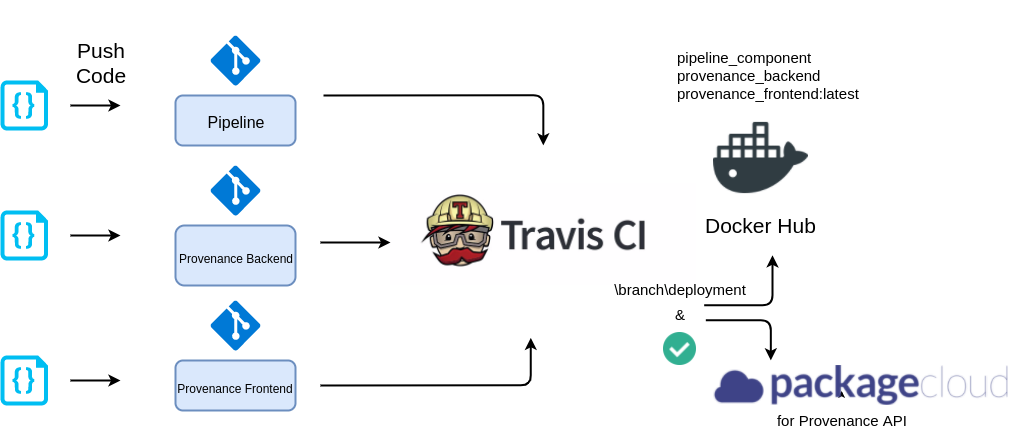
\includegraphics[width=\textwidth]{figures/deployment.png}
	\caption{Deployment Pipeline}
	\label{fig:deployment}
\end{figure}


We used Travis CI\footnote{\url{https://travis-ci.org/Krymnos/IDP}} as Continuous Integration Solution that is free for Open-Source Projects. Travis builds were triggered on changes for every branch of the repository that contains a valid \emph{travis.yaml}.
The testing configuration was set inside of the \emph{travis.yaml} that was present in each repository. Some components needed additional configuration to get builds and tests running. For example, the Pipeline Component needs the protobuf executables to generate the communication interfaces during a build. After a the compilation is finished, the unit tests of the Pipeline requires a running \emph{Redis}-Database as local storage. All these configurations could be made by the \texttt{before-script} and \texttt{before-install} sections inside the \texttt{travis.yaml} by using the built-in services of travis\footnote{\url{https://docs.travis-ci.com/user/database-setup/}}. As an example, the travis.yaml for the pipeline component can be found in the appendix \ref{lst:pipelineyaml}.
At the same file a \emph{deployment}-section was defined and only executed if the branchname is equal to "deployment". For the components that are delivered as docker builds, the respective docker deployment script was executed \ref{lst:dockerdeploy}, for the Provenance API that is included by the Pipeline Component, the artifacts was pushed to our Maven Repository\footnote{\url{https://packagecloud.io/gerritja/IDP}}. The docker deployment script pushed the docker images to \emph{Docker Hub}-Repository of our project\footnote{\url{https://hub.docker.com/r/cloudproto/}}.

\paragraph*{Docker Images}
We decided to use Docker for the deployment of our components because a docker container runs platform independent, isolated, lightweight and can be interconnect with other services in a very simple way \footnote{\url{https://docs.docker.com/engine/docker-overview/\#docker-engine}}. The docker engine (in combination wirh docker-compose or Docker Swarm) also supports a good functionality to bring a deployment to a large scale. We felt, that is exactly what we want to do with our system in later tests.

To deploy our components as Docker images, we added a \emph{Dockerfile} to Pipeline, Backend and Frontend components. A Dockerfile\footnote{\url{https://docs.docker.com/engine/reference/builder/}} contains the instuction that are executed during a build of an image. As well it's defined in a Dockerfile which commands has to be executed on an instantiation of a Container. For the Pipeline Component, for example, we specified that every instance has a Redis Database running that was started inside the docker container as a local daemon.

To make the Docker Container configurable, we introduced environment variables for the Provenance API and further settings. Also delaying the runtime of the Pipeline Component (\texttt{STARTUP\_DELAY}) is possible because we noticed that we had undesired failures at startup because depedent components were not available due a longer instantiaion phase\footnote{for example, the cassandra database takes usually more time to be available than a lightweight pipeline component}. As an example, the Dockerfile for the pipeline component can be found in the Appendix (\ref{lst:pipelinedockerfile}).





\subsection{Local and AWS Deployment}






\begin{itemize}
	\item how did we include the workload data
	\item first approach : integrate mount of S3 into the docker image (failed)
	\item second approach : implement 
	
	\item difference between compose and stack \url{https://vsupalov.com/difference-docker-compose-and-docker-stack/}
\end{itemize}



\begin{itemize}
	\item additional/manual docker deployments: sensor, goofys
\end{itemize}
